% Template for Cogsci submission with R Markdown

% Stuff changed from original Markdown PLOS Template
\documentclass[10pt, letterpaper]{article}

\usepackage{cogsci}
\usepackage{pslatex}
\usepackage{float}
\usepackage{caption}

% amsmath package, useful for mathematical formulas
\usepackage{amsmath}

% amssymb package, useful for mathematical symbols
\usepackage{amssymb}

% hyperref package, useful for hyperlinks
\usepackage{hyperref}

% graphicx package, useful for including eps and pdf graphics
% include graphics with the command \includegraphics
\usepackage{graphicx}

% Sweave(-like)
\usepackage{fancyvrb}
\DefineVerbatimEnvironment{Sinput}{Verbatim}{fontshape=sl}
\DefineVerbatimEnvironment{Soutput}{Verbatim}{}
\DefineVerbatimEnvironment{Scode}{Verbatim}{fontshape=sl}
\newenvironment{Schunk}{}{}
\DefineVerbatimEnvironment{Code}{Verbatim}{}
\DefineVerbatimEnvironment{CodeInput}{Verbatim}{fontshape=sl}
\DefineVerbatimEnvironment{CodeOutput}{Verbatim}{}
\newenvironment{CodeChunk}{}{}

% cite package, to clean up citations in the main text. Do not remove.
\usepackage{cite}

\usepackage{color}

% Use doublespacing - comment out for single spacing
%\usepackage{setspace}
%\doublespacing


% % Text layout
% \topmargin 0.0cm
% \oddsidemargin 0.5cm
% \evensidemargin 0.5cm
% \textwidth 16cm
% \textheight 21cm

\title{Preserved Structure Across Vector Space Representations}

\usepackage{lipsum}
\usepackage[utf8]{inputenc}

\author{{\large \bf Andrei Amatuni} \\ \texttt{andrei.amatuni@duke.edu} \\ Department of Psychology \\ Duke University \And {\large \bf Elika Bergelson} \\ \texttt{elika.bergelson@duke.edu} \\ Department of Psychology \\ Duke University}

\begin{document}

\maketitle

\begin{abstract}
We find evidence of preserved structure between vector space
representations of words and their corresponding image embeddings. This
is evidence of regularity between the representations learned using
distributional statistics of words and the visual characteristics of
those same items. We find that some classes of objects, namely inanimate
ones, preserve their within-class structure across these two spaces more
strongly than others (e.g.~animate objects), and that this quality of
preserving class-level relationships across representational spaces
might aid in lexical acquisition, with invariance serving as an
informative marker of category boundaries. Our current analysis does not
show significant age-of-acquisition benefits for inanimate objects, but
does exhibit a stable pattern suggesting that other partitioning schemes
might be worth exploring (or something like that)

\textbf{Keywords:}
vector space models; semantic similarity; word learning
\end{abstract}

\section{Introduction}\label{introduction}

Infants are presented with a challenge to carve the world into distinct
lexical entities in the process of learning their first language.
They're provided with little supervision while mapping a territory which
William James (1890) dubbed a ``great blooming, buzzing confusion''. How
they determine which aspects of the world to attend to in service of
this goal, is an area of ongoing research (Mareschal \& Quinn, 2001).
Different features of objects and their environments are varyingly
informative with regards to object segmentation and category structure.
Some researchers have suggested that categorization is along
fundamentally perceptual grounds and that only later in development is
conceptual knowledge incorporated into these nascent perceptual
categories (Quinn \& Eimas, 1997, 2000; Quinn, Johnson, Mareschal,
Rakison, \& Younger, 2000). Others suggest that there are in fact two
distinct processes at work, such that perceptual categories are computed
automatically by the sensory systems, while conceptual categories are
independently formed through conscious action (Mandler, 2000). Träuble
and Pauen (2007) provide evidence of functional information (regarding
the animacy of objects) influencing early category judgements. Gelman
and Markman (1986) explicitly set these two sources of category cues
against each other (i.e.~functional vs.~perceptual), in hopes of
discovering which holds greater influence in infant categorization
behavior.

The degree to which these two sources of information are separable is an
important open question. Any model which hopes to explain the mechanics
of human categorization must address how these seemingly disparate forms
of information interface in mental representations, and to what degree
they interact. In our current study we examine the degree of interaction
between representations learned by two different algorithms which
operate on apparently dissimilar inputs, namely images and text. These
algorithms learn feature representations as an unsupervised byproduct of
their particular training objectives, which are completely divorced from
one another and which may themselves be supervised. The features they
learn serve as the basis for their subsequent use towards practical ends
(e.g.~machine translation or object recognition in images).

\section{Methods}\label{methods}

We generate two sets of vector representations for a common set of words
first learned by most infants. The first set of vectors are taken from a
pretrained set of GloVe representations (Pennington, Socher, \& Manning,
2014), a modern distributional semantic vector space model. The second
set is taken from the final layer activations of a pretrained image
recognition model, Google's Inception V3 convolutional neural network
(Szegedy, Vanhoucke, Ioffe, Shlens, \& Wojna, 2016). Both of these
representations are what's refered to as ``embeddings''. They map
objects from one medium (e.g.~images or words) into a metric space where
distances between points can be computed and function as a measure of
similarity between objects.

In the case of our word vectors, the GloVe algorithm instantiates the
distributional hypothesis, which proposes that words which co-occur with
each other share similar meaning (Firth, 1957; Harris, 1954), and by
capturing the covariance of tokens in large text corpora, you capture
some aspect of their semantic structure. The image embeddings, on the
other hand, are taken from the final layer of activations in a
convolutional neural network, whose objective function tunes network
parameters in service of object recognition, where the loss function is
computed in reference to a set of labeled training images (Russakovsky
et al., 2015). The final layer of this network encodes the most abstract
and integrated visual features, serving as the basis for classification
into 1000 different classes.

\subsection{Defining a prototypical
image}\label{defining-a-prototypical-image}

In the case of word vectors, each word is assigned a unique point in a
common vector space. Different images containing objects of the same
type, on the other hand, will have varying vector representations after
passing through the layers of a neural network. This presents a problem
in comparing the two forms of representation. We must first define the
most prototypical (or average) image vector for any given category of
object.

Given a set of images \(S_c\) containing objects belonging to a single
category \(c\) (e.g.~cat, dog, chair), we define our prototypical vector
\(\hat{x}_c\) of \(S_c\) as the generalized median within a
representational space \(U\). This is the vector with minimal sum of
distances between it and all the other members of set \(S_c\) in \(U\).
If \(x\) and \(y\) are vectors in space \(U\), products of images in
\(S_c\) being passed through a neural network, then

\[
 \hat{x_c} = \operatorname*{arg\,min}_{x\in U} \sum_{y\in U} d(x, y)
\] We define our \(d(x, y)\) to be the cosine similarity measure:

\[
d(x, y) = 1 - \frac{x\cdot y}{\|x\|\|y\|}
\]

Our \(d(x, y)\) is not a metric in the strict sense, but is less
susceptible to differences in \(L^2\) norm influencing our measure of
similarity, as is the case with the Euclidean distance. These magnitude
difference can be the product of frequency effects in the training data,
and the cosine similarity corrects for this.

The image inputs we use are all 960x960 images of a single object on a
gray background. These images were chosen by virtue of their presence in
infants' early linguistic environment, aggregated as part of the
SEEDLingS project, which gathered longitudinal audio and video data of
infants' home environments (Bergelson, 2016a, 2016b). We arrive at a set
of 27 unique words, selected on the basis of having at least 9 unique
images with which to determine the most prototypical. The more images we
have of any given category, the more robust our measure of category
variance in image vector space, resulting in more representative
category vectors. These are all words found on WordBank (Frank,
Braginsky, Yurovsky, \& Marchman, 2017), a compilation of the
MacArthur-Bates Communicative Development Inventory, which we use as our
proxy for age of acquisition. By studying the behavior of these
developmentally salient objects, our analysis is able to speak to the
statistical structure of those objects which infants will be most
readily contending with.

\subsection{Comparing spaces}\label{comparing-spaces}

After we have our two sets of vectors (i.e.~those from word vector space
and those from image vector space), we can compare all the pairwise
distances between objects, both within a single space and across the
two. When comparing across the two spaces, a correlation in pairwise
distances implies that inter-object distances have been conserved. For
example, if ``dog'' and ``cat'' are close together in word space and
mutually far apart from ``chair'' and ``table'' in that same space,
maintaining this relationship for all pairwise distances in the
\textit{other} vector space means that the global inter-object structure
is preserved across this mapping, despite being in radically different
spaces, both in terms of dimensionality (300 for words, and 2048 for
images in our case) and by virtue of using completely different
algorithms and inputs to establish the vector representations for
objects. So while their absolute locations might have been radically
transformed, this correlation would be a measure of the
\textit{degree of invariance} in their positioning relative to each
other.

\section{Results}\label{results}

We find that pairwise cosine distances between objects in word vector
space correlate with those same pairwise distances in the image vector
space (see Figure \ref{fig:pairwise-corr}). If we partition the set of
inter-word distances into those that are either animate-animate,
inanimate-inanimate, or mixed, we find that the pairs of distances
between inanimate objects significantly correlate across our two spaces
(\(R = 0.38\), \(p < 1.7e-07\)), while the other two pairings do not
(see Figure \ref{fig:pairwise-corr-animate-vs-not}). We expect that
those classes of objects which preserve their structure between
representations more strongly would result in earlier object-referent
mappings. This is because inferences about object-referent mappings
conditioned on both visual and semantic features would be more stable
compared to those cases where the two representations vary
independently. For example, an object that is both round (i.e.~visual
feature) and tends to roll (i.e.~semantic feature) would be more salient
as a distinct entity than an object whose visual features are entirely
uninformative about its functional or semantic qualities.

In our current analysis the class of objects which displays stronger
structure preservation (within class) are the inanimate objects. When we
partition our set of 27 words into animate and inanimates and plot their
relative AoA, we find a noticable though insignificant preference for
inanimates (see Figures \ref{fig:animacy-aoa-prod} and
\ref{fig:animacy-aoa-comp}). The choice to partition our set into these
two categories is to a degree arbitrary, and we have no reason to
believe infants would learn one class of objects earlier than the other.
Our current analysis is offered purely as an exploratory exercise,
suggesting that perhaps partitions along other taxonomic or associative
lines may provide insight in future investigations.

\begin{CodeChunk}
\begin{figure}[tb]
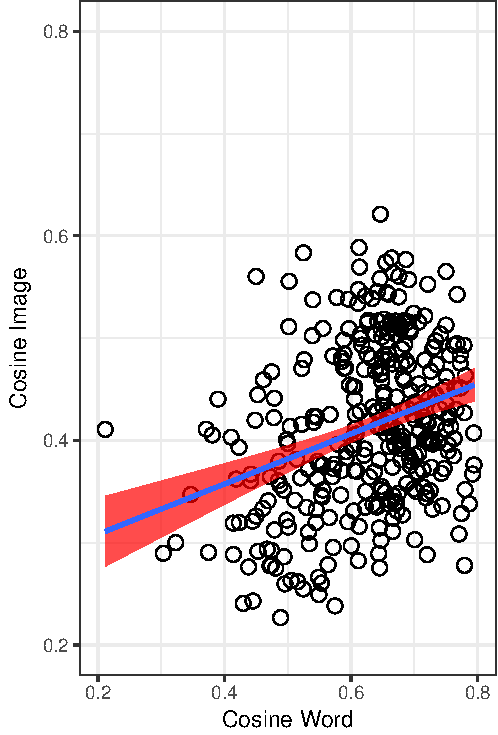
\includegraphics{figs/pairwise-corr-1} \caption[Relative cosine distance between points in word embedding space correlates with relative distance in image embedding space ($R = 0.30$, $p < 9.9e-16$)]{Relative cosine distance between points in word embedding space correlates with relative distance in image embedding space ($R = 0.30$, $p < 9.9e-16$). Graph contains all pairwise distances for every word.}\label{fig:pairwise-corr}
\end{figure}
\end{CodeChunk}

\begin{CodeChunk}
\begin{figure}[tb]
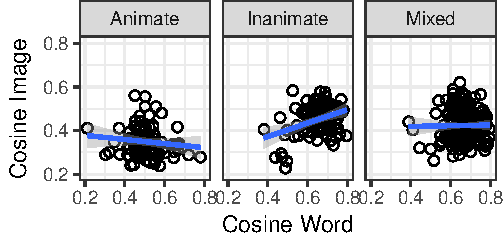
\includegraphics{figs/pairwise-corr-animate-vs-not-1} \caption[Inanimate objects display a significantly stronger correlation when mapping across vector spaces, meaning that they preserve their within-class structural relationships more reliabily across these two spaces]{Inanimate objects display a significantly stronger correlation when mapping across vector spaces, meaning that they preserve their within-class structural relationships more reliabily across these two spaces. Animate and mixed distances do not correlate. Each graph contains all pairwise distances between objects that are either a) both animate ($R = -0.13$, $p < 0.12$), b) both inanimate ($R = 0.38$, $p < 1.7e-07$), or c) mixed animate-to-inanimate ($R = -0.01$, $p < 0.8$)}\label{fig:pairwise-corr-animate-vs-not}
\end{figure}
\end{CodeChunk}

\begin{CodeChunk}
\begin{figure}[tb]
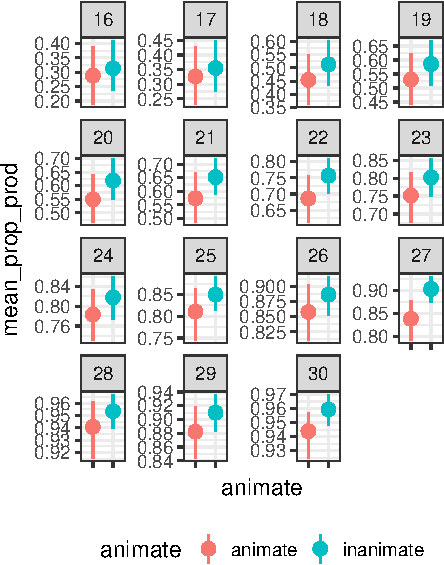
\includegraphics{figs/animacy-aoa-prod-1} \caption[By-month AoA of animates vs]{By-month AoA of animates vs. inanimates using child production data}\label{fig:animacy-aoa-prod}
\end{figure}
\end{CodeChunk}

\begin{CodeChunk}
\begin{figure}[tb]
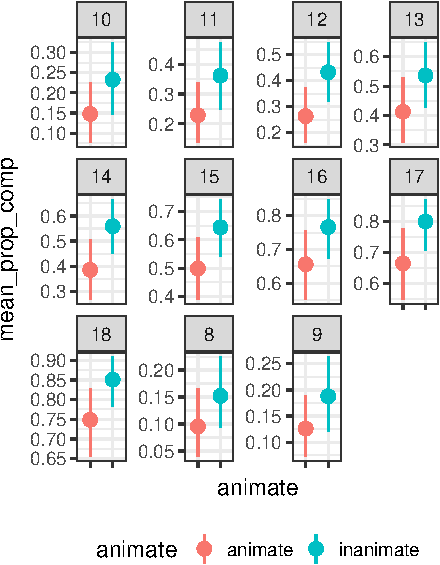
\includegraphics{figs/animacy-aoa-comp-1} \caption[By-month AoA of animates vs]{By-month AoA of animates vs. inanimates using child comprehension data}\label{fig:animacy-aoa-comp}
\end{figure}
\end{CodeChunk}

\begin{CodeChunk}
\begin{figure}[tb]
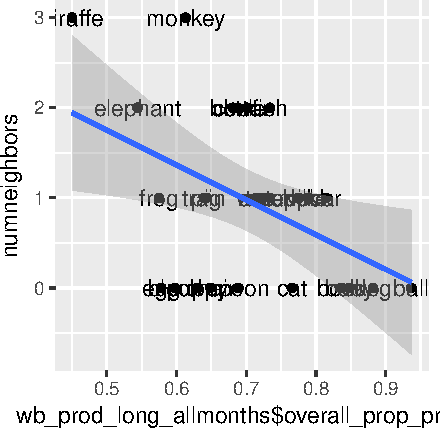
\includegraphics{figs/animacy_aoa_overall-1} \caption[AoA for animates vs inanimates collapsed over month]{AoA for animates vs inanimates collapsed over month}\label{fig:animacy_aoa_overall1}
\end{figure}
\begin{figure}[tb]
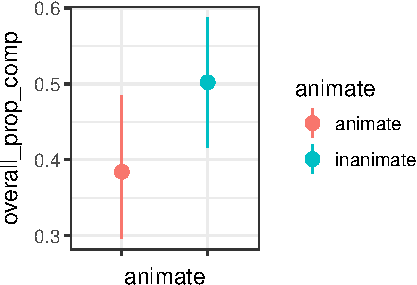
\includegraphics{figs/animacy_aoa_overall-2} \caption[AoA for animates vs inanimates collapsed over month]{AoA for animates vs inanimates collapsed over month}\label{fig:animacy_aoa_overall2}
\end{figure}
\begin{figure}[tb]
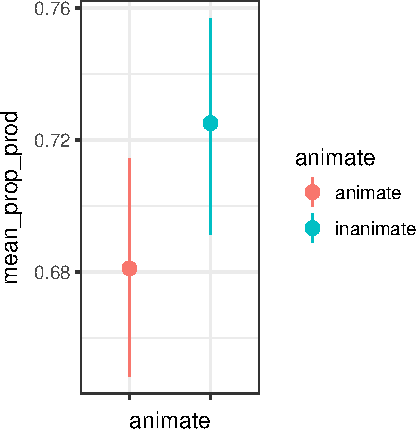
\includegraphics{figs/animacy_aoa_overall-3} \caption[AoA for animates vs inanimates collapsed over month]{AoA for animates vs inanimates collapsed over month}\label{fig:animacy_aoa_overall3}
\end{figure}
\begin{figure}[tb]
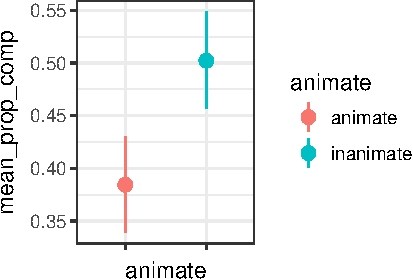
\includegraphics{figs/animacy_aoa_overall-4} \caption[AoA for animates vs inanimates collapsed over month]{AoA for animates vs inanimates collapsed over month}\label{fig:animacy_aoa_overall4}
\end{figure}
\end{CodeChunk}

\section{Discussion}\label{discussion}

\section{Conclusion}\label{conclusion}

\section{Acknowledgements}\label{acknowledgements}

Place acknowledgments (including funding information) in a section at
the end of the paper.

(Gelman \& Markman, 1986, Tversky (1977), Kemp, Bernstein, \& Tenenbaum
(2005), Hahn, Chater, \& Richardson (2003), Pennington et al. (2014),
Szegedy et al. (2016), Firth (1957), Harris (1954), Russakovsky et al.
(2015))

\section{References}\label{references}

\setlength{\parindent}{-0.1in} \setlength{\leftskip}{0.125in} \noindent

\hypertarget{refs}{}
\hypertarget{ref-bergelson2016seedlings}{}
Bergelson, E. (2016a). Bergelson seedlings homebank corpus.
\url{http://doi.org/10.21415/T5PK6D}

\hypertarget{ref-bergelson2016seedlingsdatabrary}{}
Bergelson, E. (2016b). SEEDLingS corpus. Retrieved January 26, 2018,
from \url{https://nyu.databrary.org/volume/228}

\hypertarget{ref-firth1957synopsis}{}
Firth, J. R. (1957). A synopsis of linguistic theory, 1930-1955.
\emph{Studies in Linguistic Analysis}.

\hypertarget{ref-frank2017wordbank}{}
Frank, M. C., Braginsky, M., Yurovsky, D., \& Marchman, V. A. (2017).
Wordbank: An open repository for developmental vocabulary data.
\emph{Journal of Child Language}, \emph{44}(3), 677--694.

\hypertarget{ref-gelman1986categories}{}
Gelman, S. A., \& Markman, E. M. (1986). Categories and induction in
young children. \emph{Cognition}, \emph{23}(3), 183--209.

\hypertarget{ref-hahn2003similarity}{}
Hahn, U., Chater, N., \& Richardson, L. B. (2003). Similarity as
transformation. \emph{Cognition}, \emph{87}(1), 1--32.

\hypertarget{ref-harris1954distributional}{}
Harris, Z. S. (1954). Distributional structure. \emph{Word},
\emph{10}(2-3), 146--162.

\hypertarget{ref-james2013principles}{}
James, W. (1890). \emph{The principles of psychology}. Henry Holt;
Company.

\hypertarget{ref-kemp2005generative}{}
Kemp, C., Bernstein, A., \& Tenenbaum, J. B. (2005). A generative theory
of similarity. In \emph{Proceedings of the 27th annual conference of the
cognitive science society} (pp. 1132--1137).

\hypertarget{ref-mandler2000perceptual}{}
Mandler, J. M. (2000). Perceptual and conceptual processes in infancy.
\emph{Journal of Cognition and Development}, \emph{1}(1), 3--36.

\hypertarget{ref-mareschal2001categorization}{}
Mareschal, D., \& Quinn, P. C. (2001). Categorization in infancy.
\emph{Trends in Cognitive Sciences}, \emph{5}(10), 443--450.

\hypertarget{ref-pennington2014glove}{}
Pennington, J., Socher, R., \& Manning, C. (2014). Glove: Global vectors
for word representation. In \emph{Proceedings of the 2014 conference on
empirical methods in natural language processing (emnlp)} (pp.
1532--1543).

\hypertarget{ref-quinn1997reexamination}{}
Quinn, P. C., \& Eimas, P. D. (1997). A reexamination of the
perceptual-to-conceptual shift in mental representations. \emph{Review
of General Psychology}, \emph{1}(3), 271.

\hypertarget{ref-quinn2000emergence}{}
Quinn, P. C., \& Eimas, P. D. (2000). The emergence of category
representations during infancy: Are separate perceptual and conceptual
processes required? \emph{Journal of Cognition and Development},
\emph{1}(1), 55--61.

\hypertarget{ref-quinn2000understanding}{}
Quinn, P. C., Johnson, M. H., Mareschal, D., Rakison, D. H., \& Younger,
B. A. (2000). Understanding early categorization: One process or two?
\emph{Infancy}, \emph{1}(1), 111--122.

\hypertarget{ref-ILSVRC15}{}
Russakovsky, O., Deng, J., Su, H., Krause, J., Satheesh, S., Ma, S.,
\ldots{} Fei-Fei, L. (2015). ImageNet Large Scale Visual Recognition
Challenge. \emph{International Journal of Computer Vision (IJCV)},
\emph{115}(3), 211--252. \url{http://doi.org/10.1007/s11263-015-0816-y}

\hypertarget{ref-szegedy2016rethinking}{}
Szegedy, C., Vanhoucke, V., Ioffe, S., Shlens, J., \& Wojna, Z. (2016).
Rethinking the inception architecture for computer vision. In
\emph{Proceedings of the ieee conference on computer vision and pattern
recognition} (pp. 2818--2826).

\hypertarget{ref-trauble2007role}{}
Träuble, B., \& Pauen, S. (2007). The role of functional information for
infant categorization. \emph{Cognition}, \emph{105}(2), 362--379.

\hypertarget{ref-tversky1977features}{}
Tversky, A. (1977). Features of similarity. \emph{Psychological Review},
\emph{84}(4), 327.

\end{document}
